
%(BEGIN_QUESTION)
% Copyright 2008, Tony R. Kuphaldt, released under the Creative Commons Attribution License (v 1.0)
% This means you may do almost anything with this work of mine, so long as you give me proper credit

Et av problemene med enkel av/på-regulering er at sluttelementet kobles av og på svært ofte. Dette kan føre til slitasje og kortere levetid for komponenten.

En løsning på dette problemet er å utforme systemet med et ``gap'' eller et ``bånd'' det opererer innenfor, i stedet for ett enkelt settpunkt. I praksis betyr dette to settpunkter: et øvre og et nedre settpunkt. Dette kalles ofte av/på-regulering med differensial eller av/på-regulering med dødbånd. Her vises en enkel holdekrets for dødbåndsregulering av temperaturen i en ovn.

$$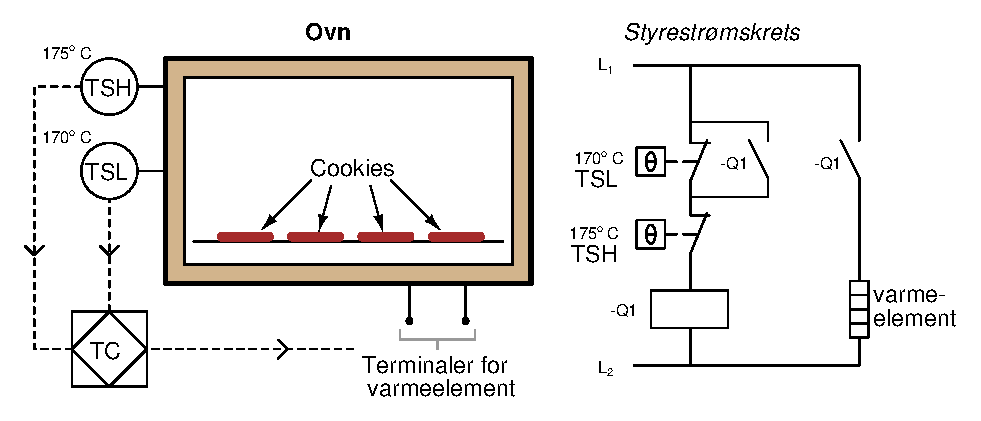
\includegraphics[width=15.5cm]{i01450x01.eps}$$

For denne ovnen betyr av/på-regulering med dødbånd at varmeelementene ikke slår seg på før temperaturen kommer under nedre settpunkt, og de slår ikke av før temperaturen går over øvre settpunkt.

$$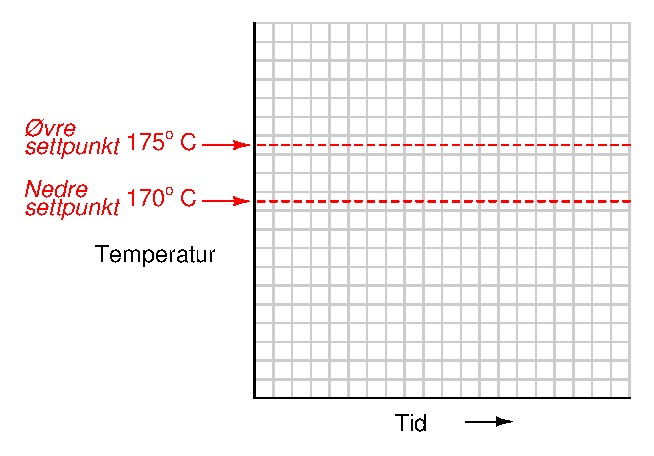
\includegraphics[width=15.5cm]{i01450x02.eps}$$

Tegn grafen for ovnens temperatur over tid når reguleringssystemet styrer den. Vis også hvordan grafen for et av/på-reguleringssystem uten dødbånd ville sett ut.

\underbar{file i01450}
%(END_QUESTION)





%(BEGIN_ANSWER)

$$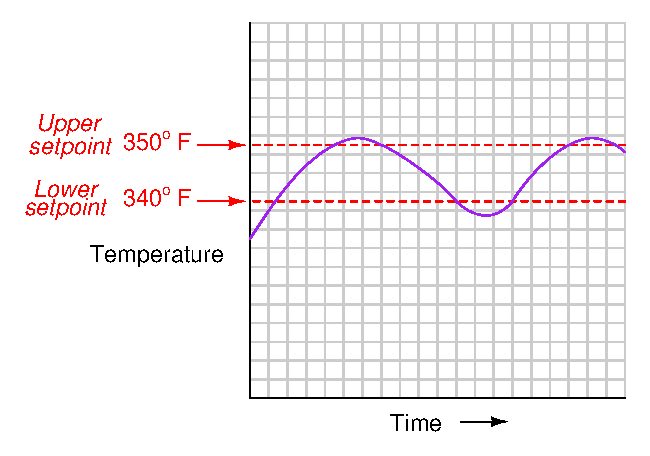
\includegraphics[width=15.5cm]{i01450x03.eps}$$

%(END_ANSWER)





%(BEGIN_NOTES)

Oppførselen til et reguleringssystem med differensialgap er en god del ``slakkere'' enn et enkelt (énpunkts) av/på-system, men i det minste sykler vi ikke sluttelementet i nærheten av like ofte.

\vskip 20pt \vbox{\hrule \hbox{\strut \vrule{} {\bf Virtuell feilsøking} \vrule} \hrule}

Dette spørsmålet egner seg godt som en ``Virtuell feilsøking''-øvelse. Når du presenterer diagrammet for studentene, forestiller du deg først en bestemt feil i systemet. Deretter presenterer du ett eller flere symptomer på denne feilen (noe en operatør eller annen bruker kan observere). Studentene foreslår så ulike diagnostiske tester for å identifisere feilens natur og plassering, slik teknikere ville gjort i praktisk feilsøking. Din oppgave er å fortelle hva resultatet ville blitt for hver foreslått test, og dokumentere resultatene slik at alle studentene kan se dem.

Under og etter øvelsen er det nyttig å stille oppfølgingsspørsmål som:

\begin{itemize}
\item{} Hva forteller resultatet av den siste diagnostiske testen deg om feilen?
\item{} Anta at resultatene av den siste diagnostiske testen var annerledes. Hva ville det resultatet fortalt deg om feilen?
\item{} Er den siste diagnostiske testen den beste vi kunne gjort?
\item{} Hva ville vært ideell testrekkefølge for å diagnostisere problemet i færrest mulig trinn?
\end{itemize}

%INDEX% Norsk
%INDEX% Control, basics: differential gap control (electromechanical relay)
%INDEX% Control, basics: on/off control (with deadband)
%INDEX% Process: cookie baking oven

%(END_NOTES)

